% Created by tikzDevice version 0.6.2 on 2012-09-11 13:10:12
% !TEX encoding = UTF-8 Unicode
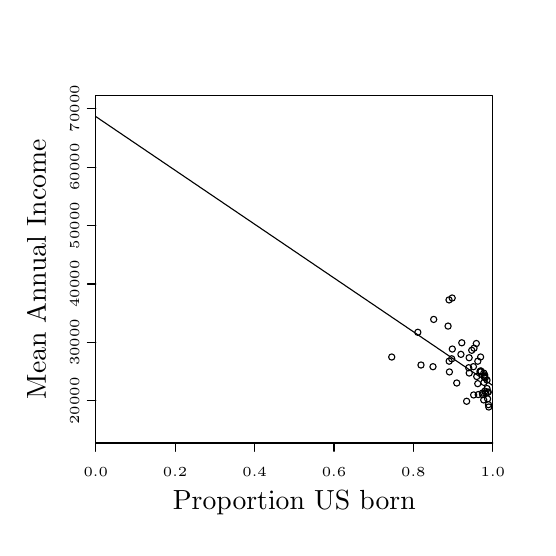
\begin{tikzpicture}[x=1pt,y=1pt,scale=0.5]
\definecolor[named]{drawColor}{rgb}{0.00,0.00,0.00}
\definecolor[named]{fillColor}{rgb}{1.00,1.00,1.00}
\fill[color=fillColor,fill opacity=0.00,] (0,0) rectangle (361.35,361.35);
\begin{scope}
\path[clip] ( 49.20, 61.20) rectangle (336.15,312.15);
\definecolor[named]{drawColor}{rgb}{0.00,0.00,0.00}

\draw[color=drawColor,line cap=round,line join=round,fill opacity=0.00,] (332.29, 97.71) circle (  2.25);

\draw[color=drawColor,line cap=round,line join=round,fill opacity=0.00,] (318.69,115.59) circle (  2.25);

\draw[color=drawColor,line cap=round,line join=round,fill opacity=0.00,] (310.09,104.55) circle (  2.25);

\draw[color=drawColor,line cap=round,line join=round,fill opacity=0.00,] (332.39, 93.08) circle (  2.25);

\draw[color=drawColor,line cap=round,line join=round,fill opacity=0.00,] (263.10,123.32) circle (  2.25);

\draw[color=drawColor,line cap=round,line join=round,fill opacity=0.00,] (320.91,128.19) circle (  2.25);

\draw[color=drawColor,line cap=round,line join=round,fill opacity=0.00,] (306.77,165.97) circle (  2.25);

\draw[color=drawColor,line cap=round,line join=round,fill opacity=0.00,] (324.24,133.08) circle (  2.25);

\draw[color=drawColor,line cap=round,line join=round,fill opacity=0.00,] (304.51,164.61) circle (  2.25);

\draw[color=drawColor,line cap=round,line join=round,fill opacity=0.00,] (292.91,116.34) circle (  2.25);

\draw[color=drawColor,line cap=round,line join=round,fill opacity=0.00,] (326.83,112.83) circle (  2.25);

\draw[color=drawColor,line cap=round,line join=round,fill opacity=0.00,] (284.24,117.55) circle (  2.25);

\draw[color=drawColor,line cap=round,line join=round,fill opacity=0.00,] (325.60, 96.19) circle (  2.25);

\draw[color=drawColor,line cap=round,line join=round,fill opacity=0.00,] (306.88,129.10) circle (  2.25);

\draw[color=drawColor,line cap=round,line join=round,fill opacity=0.00,] (329.97,109.44) circle (  2.25);

\draw[color=drawColor,line cap=round,line join=round,fill opacity=0.00,] (330.67,108.20) circle (  2.25);

\draw[color=drawColor,line cap=round,line join=round,fill opacity=0.00,] (327.38,112.66) circle (  2.25);

\draw[color=drawColor,line cap=round,line join=round,fill opacity=0.00,] (332.87, 97.98) circle (  2.25);

\draw[color=drawColor,line cap=round,line join=round,fill opacity=0.00,] (328.61, 97.30) circle (  2.25);

\draw[color=drawColor,line cap=round,line join=round,fill opacity=0.00,] (325.27,104.09) circle (  2.25);

\draw[color=drawColor,line cap=round,line join=round,fill opacity=0.00,] (313.73,133.62) circle (  2.25);

\draw[color=drawColor,line cap=round,line join=round,fill opacity=0.00,] (303.82,145.68) circle (  2.25);

\draw[color=drawColor,line cap=round,line join=round,fill opacity=0.00,] (322.13,116.36) circle (  2.25);

\draw[color=drawColor,line cap=round,line join=round,fill opacity=0.00,] (327.33,123.35) circle (  2.25);

\draw[color=drawColor,line cap=round,line join=round,fill opacity=0.00,] (333.24, 87.22) circle (  2.25);

\draw[color=drawColor,line cap=round,line join=round,fill opacity=0.00,] (330.27,110.32) circle (  2.25);

\draw[color=drawColor,line cap=round,line join=round,fill opacity=0.00,] (329.57, 92.34) circle (  2.25);

\draw[color=drawColor,line cap=round,line join=round,fill opacity=0.00,] (329.67,111.70) circle (  2.25);

\draw[color=drawColor,line cap=round,line join=round,fill opacity=0.00,] (306.45,122.04) circle (  2.25);

\draw[color=drawColor,line cap=round,line join=round,fill opacity=0.00,] (322.57,129.73) circle (  2.25);

\draw[color=drawColor,line cap=round,line join=round,fill opacity=0.00,] (293.43,150.50) circle (  2.25);

\draw[color=drawColor,line cap=round,line join=round,fill opacity=0.00,] (317.23, 91.35) circle (  2.25);

\draw[color=drawColor,line cap=round,line join=round,fill opacity=0.00,] (281.96,141.19) circle (  2.25);

\draw[color=drawColor,line cap=round,line join=round,fill opacity=0.00,] (330.15,108.67) circle (  2.25);

\draw[color=drawColor,line cap=round,line join=round,fill opacity=0.00,] (330.49, 98.69) circle (  2.25);

\draw[color=drawColor,line cap=round,line join=round,fill opacity=0.00,] (327.41,113.31) circle (  2.25);

\draw[color=drawColor,line cap=round,line join=round,fill opacity=0.00,] (328.78, 96.15) circle (  2.25);

\draw[color=drawColor,line cap=round,line join=round,fill opacity=0.00,] (319.11,111.75) circle (  2.25);

\draw[color=drawColor,line cap=round,line join=round,fill opacity=0.00,] (325.32,120.31) circle (  2.25);

\draw[color=drawColor,line cap=round,line join=round,fill opacity=0.00,] (304.59,120.33) circle (  2.25);

\draw[color=drawColor,line cap=round,line join=round,fill opacity=0.00,] (330.98, 97.15) circle (  2.25);

\draw[color=drawColor,line cap=round,line join=round,fill opacity=0.00,] (331.96,100.55) circle (  2.25);

\draw[color=drawColor,line cap=round,line join=round,fill opacity=0.00,] (331.97,106.65) circle (  2.25);

\draw[color=drawColor,line cap=round,line join=round,fill opacity=0.00,] (304.79,112.56) circle (  2.25);

\draw[color=drawColor,line cap=round,line join=round,fill opacity=0.00,] (322.30, 95.92) circle (  2.25);

\draw[color=drawColor,line cap=round,line join=round,fill opacity=0.00,] (324.53,109.26) circle (  2.25);

\draw[color=drawColor,line cap=round,line join=round,fill opacity=0.00,] (319.04,122.82) circle (  2.25);

\draw[color=drawColor,line cap=round,line join=round,fill opacity=0.00,] (313.09,125.25) circle (  2.25);

\draw[color=drawColor,line cap=round,line join=round,fill opacity=0.00,] (332.98, 88.92) circle (  2.25);

\draw[color=drawColor,line cap=round,line join=round,fill opacity=0.00,] (327.42,113.08) circle (  2.25);

\draw[color=drawColor,line cap=round,line join=round,fill opacity=0.00,] (329.75,105.00) circle (  2.25);
\end{scope}
\begin{scope}
\path[clip] (  0.00,  0.00) rectangle (361.35,361.35);
\definecolor[named]{drawColor}{rgb}{0.00,0.00,0.00}

\draw[color=drawColor,line cap=round,line join=round,fill opacity=0.00,] ( 49.20, 61.20) -- (336.15, 61.20);

\draw[color=drawColor,line cap=round,line join=round,fill opacity=0.00,] ( 49.20, 61.20) -- ( 49.20, 55.20);

\draw[color=drawColor,line cap=round,line join=round,fill opacity=0.00,] (106.59, 61.20) -- (106.59, 55.20);

\draw[color=drawColor,line cap=round,line join=round,fill opacity=0.00,] (163.98, 61.20) -- (163.98, 55.20);

\draw[color=drawColor,line cap=round,line join=round,fill opacity=0.00,] (221.37, 61.20) -- (221.37, 55.20);

\draw[color=drawColor,line cap=round,line join=round,fill opacity=0.00,] (278.76, 61.20) -- (278.76, 55.20);

\draw[color=drawColor,line cap=round,line join=round,fill opacity=0.00,] (336.15, 61.20) -- (336.15, 55.20);

\node[color=drawColor,anchor=base,inner sep=0pt, outer sep=0pt, scale=  1.00]
at ( 49.20, 37.20) {\tiny 0.0};

\node[color=drawColor,anchor=base,inner sep=0pt, outer sep=0pt, scale=  1.00] at (106.59, 37.20) {\tiny 0.2};

\node[color=drawColor,anchor=base,inner sep=0pt, outer sep=0pt, scale=  1.00] at (163.98, 37.20) {\tiny 0.4};

\node[color=drawColor,anchor=base,inner sep=0pt, outer sep=0pt, scale=  1.00] at (221.37, 37.20) {\tiny 0.6};

\node[color=drawColor,anchor=base,inner sep=0pt, outer sep=0pt, scale=  1.00] at (278.76, 37.20) {\tiny 0.8};

\node[color=drawColor,anchor=base,inner sep=0pt, outer sep=0pt, scale=  1.00] at (336.15, 37.20) {\tiny 1.0};

\draw[color=drawColor,line cap=round,line join=round,fill opacity=0.00,] ( 49.20, 91.62) -- ( 49.20,302.86);

\draw[color=drawColor,line cap=round,line join=round,fill opacity=0.00,] ( 49.20, 91.62) -- ( 43.20, 91.62);

\draw[color=drawColor,line cap=round,line join=round,fill opacity=0.00,] ( 49.20,133.87) -- ( 43.20,133.87);

\draw[color=drawColor,line cap=round,line join=round,fill opacity=0.00,] ( 49.20,176.11) -- ( 43.20,176.11);

\draw[color=drawColor,line cap=round,line join=round,fill opacity=0.00,] ( 49.20,218.36) -- ( 43.20,218.36);

\draw[color=drawColor,line cap=round,line join=round,fill opacity=0.00,] ( 49.20,260.61) -- ( 43.20,260.61);

\draw[color=drawColor,line cap=round,line join=round,fill opacity=0.00,] ( 49.20,302.86) -- ( 43.20,302.86);

\node[rotate= 90.00,color=drawColor,anchor=base,inner sep=0pt, outer sep=0pt,
scale=  1.00] at ( 37.20, 91.62) {\tiny 20000};

\node[rotate= 90.00,color=drawColor,anchor=base,inner sep=0pt, outer sep=0pt, scale=  1.00] at ( 37.20,133.87) {\tiny 30000};
\node[rotate= 90.00,color=drawColor,anchor=base,inner sep=0pt, outer sep=0pt, scale=  1.00] at ( 37.20,176.11) {\tiny 40000};
\node[rotate= 90.00,color=drawColor,anchor=base,inner sep=0pt, outer sep=0pt, scale=  1.00] at ( 37.20,218.36) {\tiny 50000};
\node[rotate= 90.00,color=drawColor,anchor=base,inner sep=0pt, outer sep=0pt, scale=  1.00] at ( 37.20,260.61) {\tiny 60000};
\node[rotate= 90.00,color=drawColor,anchor=base,inner sep=0pt, outer sep=0pt, scale=  1.00] at ( 37.20,302.86) {\tiny 70000};

\draw[color=drawColor,line cap=round,line join=round,fill opacity=0.00,] 
    ( 49.20, 61.20) --
	(336.15, 61.20) --
	(336.15,312.15) --
	( 49.20,312.15) --
	( 49.20, 61.20);
\end{scope}
\begin{scope}
\path[clip] (  0.00,  0.00) rectangle (361.35,361.35);
\definecolor[named]{drawColor}{rgb}{0.00,0.00,0.00}

\node[color=drawColor,anchor=base,inner sep=0pt, outer sep=0pt, scale=  1.00] at (192.68, 13.20) {Proportion US born};

\node[rotate= 90.00,color=drawColor,anchor=base,inner sep=0pt, outer sep=0pt, scale=  1.00] at ( 13.20,186.67) {Mean Annual Income};
\end{scope}
\begin{scope}
\path[clip] ( 49.20, 61.20) rectangle (336.15,312.15);
\definecolor[named]{drawColor}{rgb}{0.00,0.00,0.00}

\draw[color=drawColor,line cap=round,line join=round,fill opacity=0.00,] ( 49.20,297.12) -- (336.15,102.70);
\end{scope}
\end{tikzpicture}
